\section{Pulssensor med tilhørende algoritme}\label{sec_de_im_te_puls}
\textit{Dette afsnit beskriver design, implementering og test af pulssensoren og den tilhørende algoritme.}

\subsection{Design} \label{sec_design_puls}
Pulssensoren skal benyttes til at beskrive intensiteten af aktiviteten, som er beskrevet i \secref{subsub:ak_int}. Heraf kan effekten af aktiviteten bestemmes, hvilket vil blive benyttet som en motiverende faktor i forbindelse med visualisering i GUI. \newline
Pulssensoren SEN-11574 er valgt til dette projekt, da denne er en optisk pulssensor og er alsidig i forhold til placering, som beskrevet i \secref{sec:pulssensor}. En optisk sensor påkræver blot en placering over en blodåre for at kunne måle pulsen, som følge af blodets gennemstrømning. Eksempelvis kan den optiske sensor placeres på fingerspidsen eller øreflippen, hvoraf sensoren i dette projekt placeres på øreflippen. Dette skyldtes, at ved en placering på øreflippen er der mindre bevægelse af sensor og ledninger end ved en fingerspids, hvormed mængden af støj kan reduceres. \\
SEN-11574 kræver en spændingstilkobling på 3~V til 5~V for at være funktionel og forbruger 4~mA ved en forsyning på 5~V. På sensorens printplade findes et aktivt filter\fxnote{Et aktivt filter er en type af analog elektronisk filter, der anvender aktive bestanddele, såsom en forstærker.} samt en forstærker, som tilsammen øger amplituden for pulsbølgen og normaliserer signalet omkring et referencepunkt, hvilket fjerner DC spænding i signalet. \citep{Murphy2016,Murphy2016_sensor}\\
Pulssensoren designes således, at pulsen beregnes for brugeren i GAP peripheral og sendes til GAP central, hvilket fremgår af \figref{fig:puls_pseudo}.
\begin{figure}[H]
	\centering
	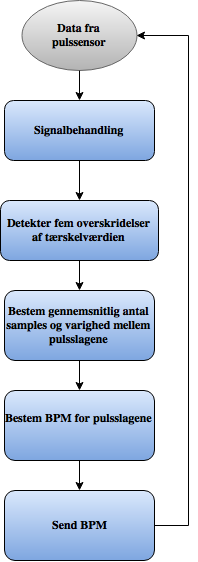
\includegraphics[scale=0.5]{figures/cDesign/Pulssensor.png}
	\caption{På figuren ses et flowchart over algortimen til detektering af puls. Pulssensorens algoritme skal registrere fem pulsslag, som overskrider en fastsat tærskelværdi, førend pulsen kan bestemmes. Pulsen sendes afslutningsvis med BLE.}
	\label{fig:puls_pseudo}
\end{figure}\vspace{-.25cm}
\Figref{fig:puls_pseudo} viser, at pulssensoren opfanger pulssignalet, hvorefter dette signal bliver signalbehandlet førend detektering af pulsslag startes. Der ønskes at detektere pulsen ved at beregne varigheden mellem fem pulsslag med udgangspunkt i det systoliske peak, hvilket fremgår af \secref{sec:pulssensor}. Dette peak har større amplitude end peaket for diastole, hvormed signalbehandlingen skal forstærke det systoliske peak og dæmpe det diastoliske peak.  \\
Dataet fra pulssensoreren signalbehandles i form af division med 32 og kvadrering. Dette vil medføre, at det største peak i signalet vil blive forøget i amplitude, og de mindre peaks vil opnå en lavere amplitude, hvilket ses på \figref{fig:behandlet_puls}. 
\begin{figure}[H]
	\centering
	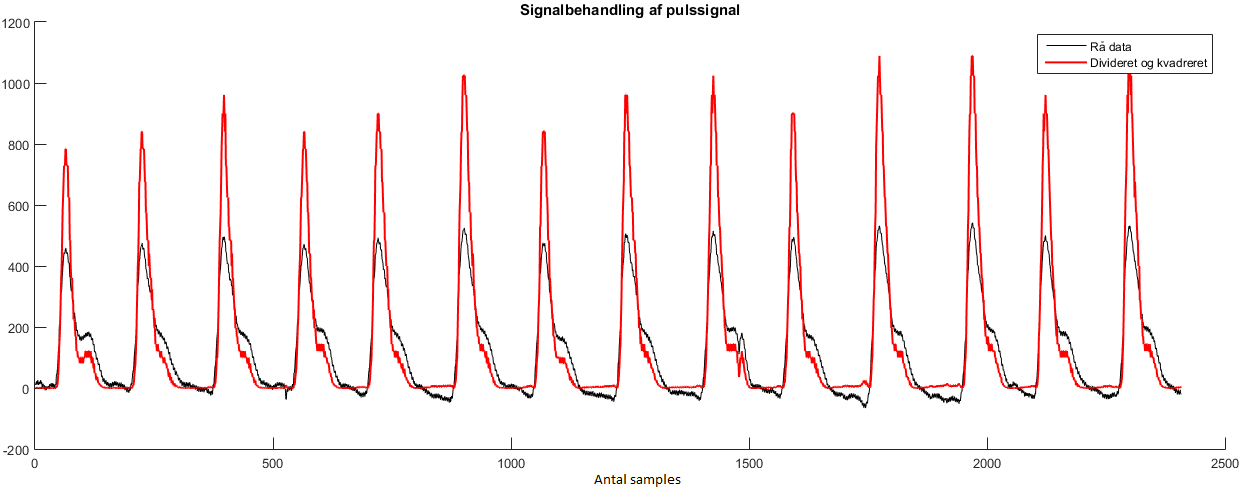
\includegraphics[scale=0.37]{figures/cDesign/puls_ore_behandlet.png}
	\caption{På figuren ses algoritmens signalbehandling af et råt pulssignal fra den optiske pulssensor. Den sorte kurve er det rå pulssignal, og den røde kurve er det dividerede og kvadrerede signal.}
	\label{fig:behandlet_puls}
\end{figure}\vspace{-.25cm}
Der ses på \figref{fig:behandlet_puls}, at resultatet af signalbehandlingen er, at amplituden på det behandlede signal er forøget, hvorimod de mindre peaks er formindsket. De største peaks i signalet repræsenterer den systoliske periode i hjertecyklussen, hvilket er det peak, der benyttes til at bestemme pulsen i signalet. For at kunne bestemme pulsen implementeres en tærskelværdi. Denne værdi skal signalet overskride og efterfølgende gå under for at blive detekteret som et systolisk peak. Tærskelværdien for algoritmen bestemmes med udgangspunkt i en pulsmåling, hvor sensoren er placeret på øreflippen. Dette fremgår af \figref{fig:taerskel_puls}.
\begin{figure}[H]
	\centering
	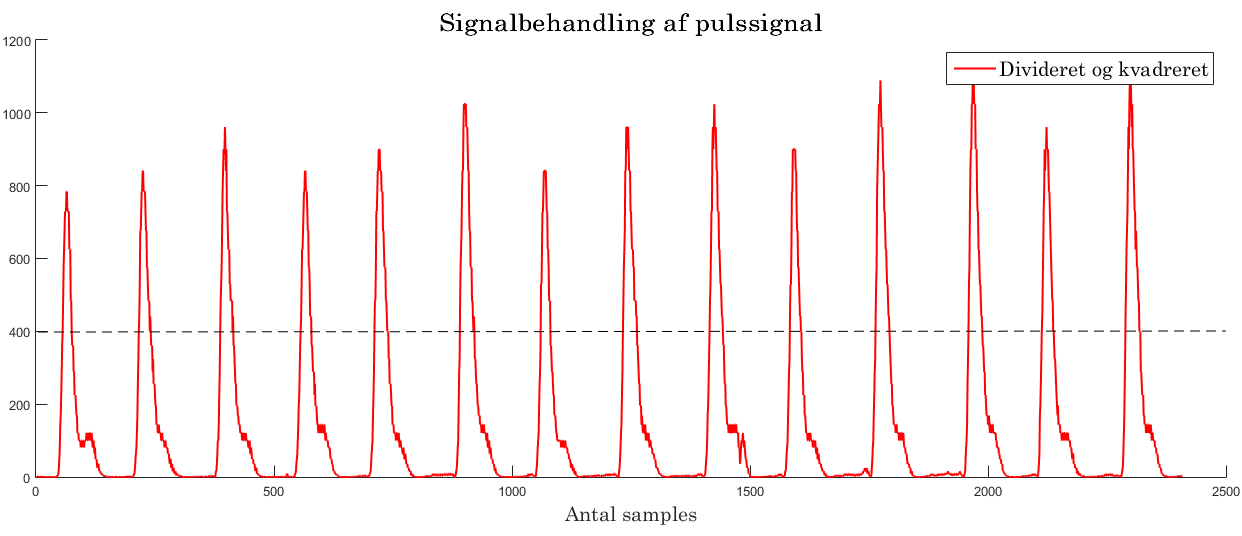
\includegraphics[scale=0.37]{figures/cDesign/puls_taerskel.png}
	\caption{På figuren ses en pulsmåling foretaget på øreflippen. Den røde kurve er en signalbehandlet pulsmåling fra øreflippen, og den sorte stiplede linje er algoritmens tærskelværdi, som har en værdi på 400.}
	\label{fig:taerskel_puls}
\end{figure}\vspace{-.25cm}
Det behandlede signal fremgår af \figref{fig:taerskel_puls}, hvor der er indtegnet en tærskelværdi på 400, som alle de systoliske peaks vil overskride. Tærskelværdi på 400 vil medføre, at det systoliske tryk overstiger tærskelværdien, hvortil det diastoliste tryk vil befinde sig under. Algoritmen vil benytte varigheden mellem de forekomne systoliske tryk til at kunne beregne pulsen med udgangspunkt i fem detekterede peaks. 

\subsection{Implementering} \label{puls_impl}
Pulssensoren har 3 pins til henholdsvis spændingsforsyning, ground og outputsignal. Disse pins kobles til hver sin pin på GAP peripheral. Outputsignalets pin skal designes i PSoC Creator, således MCUen modtager pulssensorens signaler fra den pågældende pin. Dette gøres ved at indsætte henholdsvis en UART serie kommunikationsblok (SCB) og SAR ADC i topdesignet. UARTen bruges til kommunikation mellem sensor og MCU. Standardindstillingerne for denne blok benyttes til konfigurationen af MCUen. \newline
Outputsignalet fra sensoren er et analogt signal, hvormed dette signal samples af en ADC for at skabe en konvertering til et digitalt signal. ADCens design skal derfor konfigureres således, at denne bearbejder én single ended input fra pulssensoren. Yderligere indstilles samplingsfrekvensen for ADCen for den pågældende inputkanal til 35~Hz i forhold til \secref{krav_adc}. \\
Efter konfigurering af UART og ADC i topdesignet skal de korrekte pins indstilles i pinopsætning. UART tildeles interne RX-, og TX-pins, hvorimod ADCens inputpin skal indstilles til den pin, som outputtet fra sensoren er placeret i, hvilket er valgt til pin 2.0. \\
Med udgangspunkt i ovenstående elementer bliver der implementeret en algoritme til pulsdetekteringen, som det ses på \figref{fig:puls_pseudo_c}.
\begin{figure}[H]
	\centering
	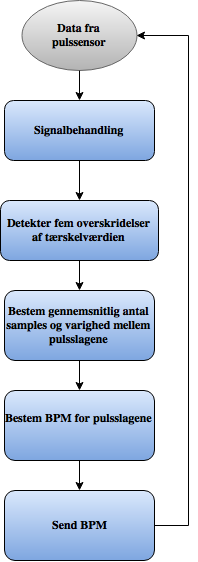
\includegraphics[scale=0.4]{figures/cDesign/Pulssensor.png}
	\caption{På figuren ses et flowchart over pulssensorens algoritme udført i C kode. Data fra pulssensoren AD konverteres, hvorefter en signalbehandling muliggør en detektering af pulsen. Afslutningsvis sendes den beregnede puls med BLE og benyttede variabler nulstilles. Når data er klar, startes proceduren forfra.}
	\label{fig:puls_pseudo_c}
\end{figure} \vspace{-.25cm}
Første trin efter dataopsamlingen fra pulssensoren er en konvertering af det analoge signal til et digitalt. Derefter undersøges det, hvorvidt det konverterede data er klar, hvortil en indbygget kodegenerering benyttes, hvilken yderligere beskrives i \secref{adc_design_impl}. Hvis data er klar, signalbehandles dataet med division og kvadrering, som beskrevet i design. Herefter starter algoritmens time counter, der starter optælling af samples. Den behandlede sample gemmes i en variabel 'Value[0]'. Når der kommer en ny sample, vil den forrige sample blive gemt i en ny variabel 'Value[1]', og den nye sample gemmes på ny plads i arrayet for 'Value[0]'. Yderligere tæller algoritmen antallet af pulsslag ved at vurdere, om 'Value[0]' er under tærkselværdien og 'Value[1]' er over. Hvis dette er tilfældet, vil der blive lagt én til antal pulsslag, dog maksimalt til antal pulsslag er mindre end 6. Algoritmen er bestemt til at nulstille sin time counter, hver gang der registreres fem tilfælde, hvor en sample er gået over og under tærskelværdien på 400. Derfor vil algoritmen kunne beregne pulsen for brugeren med det forbehold, at antallet af detekterede pulsslag skal være fem. Time counteren benyttes i denne forbindelse til at optælle antallet af samples for fem pulsslag. Beregningen foretages ved at bestemme den gennemsnitlige varighed mellem hvert pulsslag med udgangspunkt i fem pulsslag. Derefter divideres denne varighed med 60 sekunder for at kunne bestemme puls. Når beregningen er foretaget, vil pulsen for brugeren blive sendt til GAP central gennem BLE, hvorefter algoritmens værdier nulstilles.\\

\subsection{Test}
Pulssensoren testes for at undersøge hvorvidt den designede og implementerede algoritme kan bestemme den rigtige puls ved et simuleret signal. Ydermere testes sensoren og algoritmen ved at benytte en Vernier Excercise Heart Rate Monitor som reference for pulsen i BPM, som pulssensoren og den tilhørende algoritme bør sende via BLE. Referencen er ydeligere placeret om brystkassen som et pulsbælte. \\
Testen udføres på baggrund af de opstillede krav og tilhørende afvigelser opstillet i \secref{puls_krav}. Kravene til pulsedetektering, beskriver at pulsdetekteringen skal:
\begin{itemize}
\item Kunne detektere brugerens puls ved fysisk aktivitet. Der accepteres en afvigelse på 10\%.
\end{itemize}
Algoritmens funktionalitet testes ved at indsende et simuleret signal, som består af et absolut sinussignal. Peaks på det simulerede signal skal repræsentere de systoliske peaks i et pulssignal optaget med en pulssensor.\\
Det simulerede signal sendes ind i MCUen, hvorefter det undersøges, hvorvidt time counteren detekterer varigheden mellem signalet går under tærskelværdien på 400. Når pulsen er bestemt, benyttes programmet Realterm til at printe algoritmens slutresultat som puls i BPM. Det simulerede sinussignal har en frekvens på 0,6~Hz, en samplingsfrekvens på 35~Hz samt en længde på 992 samples. Derfor kan det bestemmes hvilken puls, som algoritmen bør printe i Realterm. \\
Der indsendes 992 samples og benyttes en samplingsfrekvens på 35~Hz, hvormed arrayet har en længde på 28,3 sekunder. Idet der er tale om et absolut sinussignal på 0,6~Hz, vil der opstå 34 peaks i det indsendte signal. Dette vil betyde, at algoritmen skal udregne og printe seks værdier for pulsen, idet der er 34 fuldstændige peaks. Når der er 34 peaks og arrayet har en varighed af 28,3 sekunder, vil der være 0,83 sekunder mellem hver overskridelse af tærskelværdien, hvormed pulsen bestemmes, som det fremgår af \eqref{eq:puls_teori}:
\begin{equation}
\frac{60~sekunder}{Varighed~mellem~samples} = \frac{60~sekunder}{0,83~sekunder} = 72~BPM
\label{eq:puls_teori}
\end{equation} 
Det indsendte signal har dermed en teoretisk værdi på 72 BPM, hvorfor det er forventeligt, at algoritmen vil beregne og printe denne puls.

Algoritmen er bestemt til at nulstille time counteren hver gang der registreres fem tilfælde, hvor en sample er gået over og under tærskelværdien. Derfor vil algoritmen gøre brug af time counterens optalte antal samples til at bestemme pulsen for den pågældende periode. \\
Ved at indsende det simulerede signal fremgår det af \figref{fig:timecounter_puls_realterm}, hvordan time counteren nulstilles, når der er registreret fem tilfælde. Ydermere ses det i \tabref{tab:test_puls_realterm}, at Realterm har printet de forventede værdier for pulsen.
\begin{figure}[H]
	\centering
	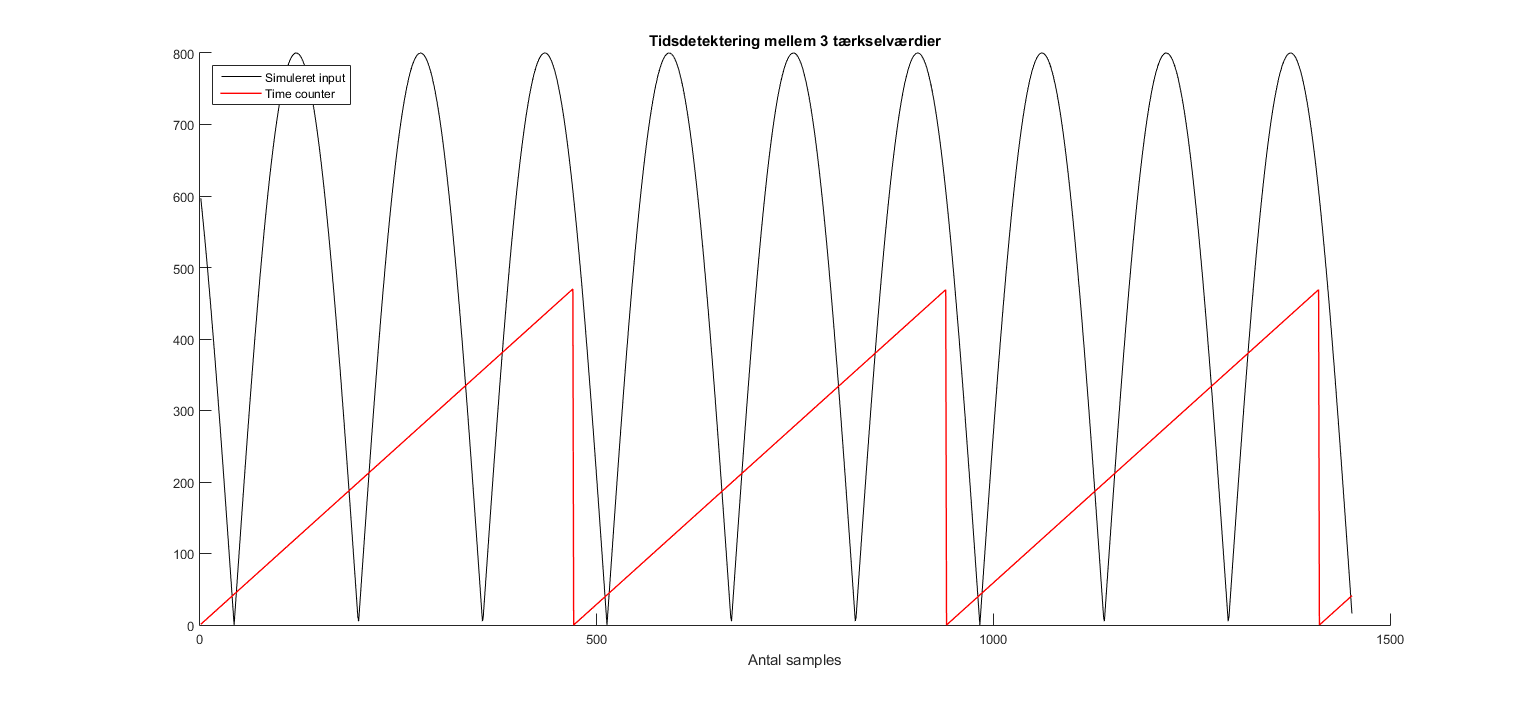
\includegraphics[scale=0.34]{figures/cDesign/timecounter_puls_pic.png}
	\caption{På figuren ses algoritmens time counter, som tæller op, indtil en sample på det femte pulsslag er gået under tærskelværdien. Efterfulgt af dette vil time counteren nulstilles og genstarte optælling af samples.}
	\label{fig:timecounter_puls_realterm}
\end{figure}\vspace{-.25cm}
Det fremgår af \figref{fig:timecounter_puls_realterm}, at algoritmen tæller indtil fem peaks er detekteret. Herefter beregner algoritmen pulsen ud fra det antal samples, som findes inden for disse fem peaksdetekteringer. Herefter printes pulsen i Realterm, som det fremgår af \tabref{tab:test_puls_realterm}.
\begin{table}[H]
	\centering
	\begin{tabular}{ccc}
		\hline
		\rowcolor[HTML]{C0C0C0} 
		Forventet værdi [BPM] & Modtaget værdi [BPM] & Afvigelse [\%]\\ \hline
		72 - 72 - 72 - 72 - 72 - 72         & 72 - 72 - 72 - 72 - 72 - 72         & 0 - 0 - 0 - 0 - 0 - 0 \\ \hline
	\end{tabular}
	\caption{I tabellen ses resultaterne fra algoritmens beregning af pulsen på et simuleret inputsignal. I 'Modtaget værdi' ses værdierne printet i Realterm.}
	\label{tab:test_puls_realterm}
\end{table} \vspace{-.25cm}
Det fremgår, at den forventede puls var 72 BPM samt at Realterm modtager og printer en tilsvarende værdi. Det kan derfor konkluders, at algoritmen har 0\% afvigelse på et simuleret inputsignal. \\
Det kan derfor konkluderes, at pulssensoren og den tilhørende algoritme fungerer som tiltænkt ved benyttelse af et simuleret inputsignal. 

Der foretages yderligere tre tests med henblik på at vurdere, hvorvidt pulssensoren opfylder de opstillede krav. Den ene test er ved en stillesiddende position, mens den anden og tredje test er ved fysisk aktivitet i form af henholdsvis gang og løb. Det er gældende for alle tests, at der bliver benyttet en pulsmåler i form af en Vernier Excercise Heart Rate Monitor, der benyttes som reference for den beregnede puls af algoritmen. Denne pulssensors data vil blive printet i programmet LoggerPro, og resultatet vedrørende pulsdetektering vil blive visualiseret i Realterm. \\
Pulssensoren og den tilhørende algoritme testes på en stillesiddende person, hvoraf personens puls er forholdsvis stabil og uden markante udsving. Testen udføres ved at have pulssensoren påført øreflippen, hvoraf MCUen bestemmer puls i BPM og visualiserer denne værdi i Realterm. \\
Resultaterne af den første udførte test, ved en stillesiddende position, fremgår af \tabref{tab:test_pulssystem}.
\begin{table}[H]
	\centering
\begin{tabular}{ccc}
	\hline
	\cellcolor[HTML]{C0C0C0}\begin{tabular}[c]{@{}c@{}}Gennemsnitspuls \\ LoggerPro {[}BPM{]}\end{tabular} & \cellcolor[HTML]{C0C0C0}\begin{tabular}[c]{@{}c@{}}Gennemsnitspuls \\ algoritme {[}BPM{]}\end{tabular} & \cellcolor[HTML]{C0C0C0}\begin{tabular}[c]{@{}c@{}}Afvigelse \\ {[}\%{]}\end{tabular} \\ \hline
	60 & 64,9 & 8,15 \\ \hline
\end{tabular}
	\caption{I tabellen ses det den gennemsnitlige puls fra LoggerPro og Realterm målt på stillesiddende person.}
	\label{tab:test_pulssystem}
\end{table}\vspace{-.25cm}
Det fremgår af \tabref{tab:test_pulssystem}, at testen af pulssensoren og den tilhørende algoritme viser en gennemsnitlig afvigelse fra referenceværdien på 8,15\%. Pulssensoren og den tilhørende algoritme overholder dermed første krav til pulsdetekteringen, ved stillesiddende position.

Anden test undersøger hvorvidt det er muligt at detektere puls under fysisk aktivitet. Denne test indebærer en pulsmåling under fysisk aktivitet i form af gang ved 4,8~km/t på et løbebånd.\\
Resultaterne af den anden udførte test med gang, fremgår af \tabref{tab:test_puls_aktivitet}.
\begin{table}[H]
	\centering
	\begin{tabular}{ccc}
		\hline
		\cellcolor[HTML]{C0C0C0}\begin{tabular}[c]{@{}c@{}}Gennemsnitspuls \\ LoggerPro {[}BPM{]}\end{tabular} & \cellcolor[HTML]{C0C0C0}\begin{tabular}[c]{@{}c@{}}Gennemsnitspuls \\ algoritme {[}BPM{]}\end{tabular} & \cellcolor[HTML]{C0C0C0}\begin{tabular}[c]{@{}c@{}}Afvigelse \\ {[}\%{]}\end{tabular} \\ \hline
		116,5 & 95,70 & -17,85 \\ \hline
	\end{tabular}
	\caption{I tabellen ses det den gennemsnitlige puls fra LoggerPro og Realterm ved gang.}
	\label{tab:test_puls_aktivitet}
\end{table}\vspace{-.25cm}
Det fremgår af \tabref{tab:test_puls_aktivitet}, at testen af pulssensoren og den tilhørende algoritme under gang ved 4,8~km/t viser en gennemsnitlig afvigelse fra referenceværdien på -17,85\%. Pulsdetekteringen ved gang overholder derfor ikke det opstillede krav for pulsdetektering under aktivitet.\\
Yderligere testes pulsdetektering ved løb med 11,3~km/t på samme vis som foregående tests. Resultaterne af den sidste udførte test, fremgår af \tabref{tab:test_puls_aktivitet_run}.
\begin{table}[H]
	\centering
	\begin{tabular}{ccc}
		\hline
		\cellcolor[HTML]{C0C0C0}\begin{tabular}[c]{@{}c@{}}Gennemsnitspuls \\ LoggerPro {[}BPM{]}\end{tabular} & \cellcolor[HTML]{C0C0C0}\begin{tabular}[c]{@{}c@{}}Gennemsnitspuls \\ algoritme {[}BPM{]}\end{tabular} & \cellcolor[HTML]{C0C0C0}\begin{tabular}[c]{@{}c@{}}Afvigelse \\ {[}\%{]}\end{tabular} \\ \hline
		154 & 82,6 & -46,4 \\ \hline
	\end{tabular}
	\caption{I tabellen ses det den gennemsnitlige puls fra LoggerPro og Realterm ved løb.}
	\label{tab:test_puls_aktivitet_run}
\end{table}\vspace{-.25cm}
Det fremgår af \tabref{tab:test_puls_aktivitet_run}, at testen af pulssensoren og den tilhørende algoritme under løb ved 11,3~km/t viser en gennemsnitlig afvigelse fra referenceværdien på -46,4\%. Pulsdetekteringen ved løb overholder derfor ikke det opstillede krav for pulsdetektering under aktivitet.

Det fremgår af de udførte tests, at pulsdetektering er funktionel ved et simuleret input samt ved stillesiddende positioner. Dog er afvigelsen for pulsdetektering ved henholdsvis gang og løb større end den tilladte afvigelse. Det kan derfor konkluderes, at pulsdetektering ikke er mulig at benytte under fysisk aktivitet som resultat af den tilgængelige pulssensor. Pulsdetekteringen vil derfor ikke indgå yderligere i rapporten grundet testens afvigelser.